\documentclass{article}
\usepackage[utf8]{inputenc}
\usepackage{graphicx}

\title{Reporte 3: Secuencia Fibonacci\\\textbf{Análisis de Algoritmos}}
\author{ Ramiro Estrada García\\2015190034 }
\date{22 de Octubre del 2020}

\begin{document}
\maketitle
\vspace{5cm}
\section {Características del PC}
\begin{itemize}
	\item CPU: Intel Core i5 9700F a 4.1GHz
	\item RAM: 16GB a 2666MHz
\end{itemize}
\newpage
\maketitle
\section{Iterativo vs. Recursivo}
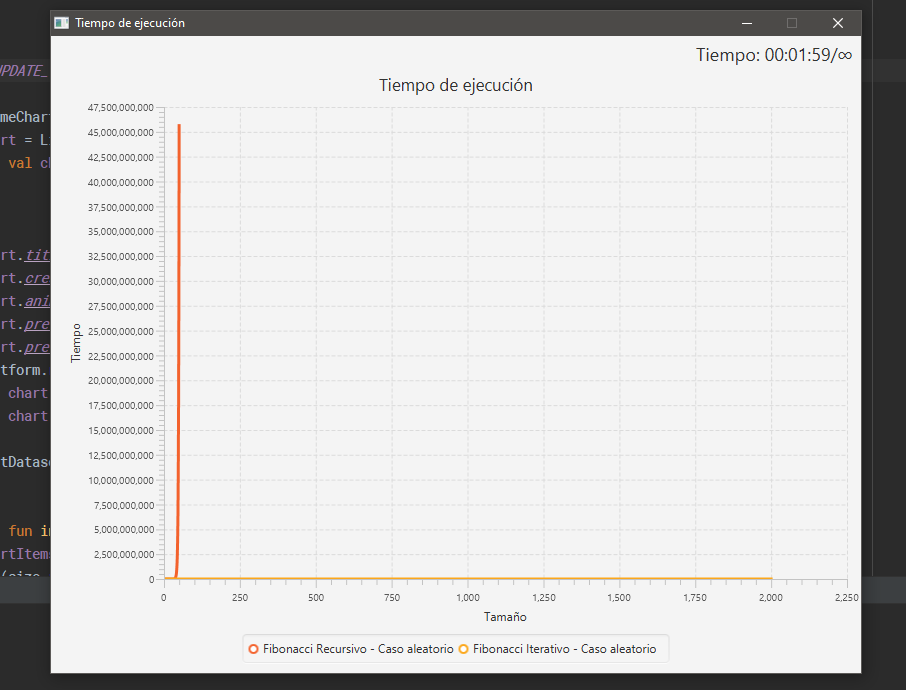
\includegraphics[width=12cm]{grafica.png}
\\ \\
El dominio de las pruebas es $[0, 2000]$ para el iterativo y de $[0, 50]$. 
La secuencia por medio de recursividad se muestra de color rojo. A partir de
aproximadamente el índice 20 empieza a crecer exponencialmente por lo que es
poco práctico mostrar más allá del índice 50 de la secuencia.\\
De color amarillo se muestra la secuencia por método iterativo. Este método
crece de manera lineal por lo que su crecimiento comparado con el recursivo
es despreciable. Para poder ver el crecimiento necesitaríamos pedir al menos
el índice 100000 de la secuencia.
\end{document}